\documentclass{article}
\usepackage[english,greek, main=greek]{babel}
\usepackage[utf8]{inputenc}
\usepackage{fullpage}

\usepackage{amsmath}
\usepackage{chngcntr}
\counterwithin{equation}{section}

\usepackage{graphicx}
\usepackage{subcaption}
\usepackage{placeins}
\usepackage{verbatim}

\usepackage{multirow}
\usepackage{xcolor}
\usepackage{listings}

\definecolor{mGreen}{rgb}{0,0.6,0}
\definecolor{mGray}{rgb}{0.5,0.5,0.5}
\definecolor{mPurple}{rgb}{0.58,0,0.82}
\definecolor{light-gray}{gray}{0.95}
\definecolor{backgroundColour}{rgb}{0.95,0.95,0.92}

\lstdefinestyle{CStyle}{
    backgroundcolor=\color{backgroundColour},   
    commentstyle=\color{mGreen},
    keywordstyle=\color{magenta},
    numberstyle=\tiny\color{mGray},
    stringstyle=\color{mPurple},
    basicstyle=\footnotesize,
    breakatwhitespace=false,         
    breaklines=true,                 
    captionpos=b,                    
    keepspaces=true,                 
    numbers=left,                    
    numbersep=5pt,                  
    showspaces=false,                
    showstringspaces=false,
    showtabs=false,                  
    tabsize=2,
    language=C
}

\lstset{language=bash, 
    basicstyle=\small\ttfamily, 
    keywordstyle=\color{blue}\bfseries, 
    commentstyle=\color{gray}, 
    stringstyle=\color{green!50!black},
    backgroundcolor=\color{light-gray},
    showstringspaces=false,
    breaklines=true,
linewidth=\textwidth}

\lstset{language=Python,
    basicstyle=\small\ttfamily,
    keywordstyle=\bfseries\color{blue},
    commentstyle=\color{gray},
    stringstyle=\color{green!50!black},
    showstringspaces=false,
breaklines=true}

\newcommand{\eng}[1]{\foreignlanguage{english}{#1}}
\newcommand{\Alpha}{\mathrm{A}}

\useshorthands{;}
\defineshorthand{;}{?}

\title{Προηγμένα Θέματα Αρχιτεκτονικής Υπολογιστών\\
\large Άσκηση 2η}
\author{Αναστάσιος Στέφανος Αναγνώστου \\
\large 03119051}

\begin{document}

\maketitle
\clearpage
\tableofcontents
\clearpage

Οι υλοποιήσεις των διαφόρων \eng{predictors} παρατίθενται στο παράρτημα στο τέλος της αναφοράς. 

\section{Μελέτη Εντολών Άλματος}

Παρατίθεται γράφημα το οποίο παρουσιάζει τα διάφορα στατιστικά στοιχεία των εντολών διακλάδωσης των μετροπρογραμμάτων:

\begin{figure}[h]
    \centering
    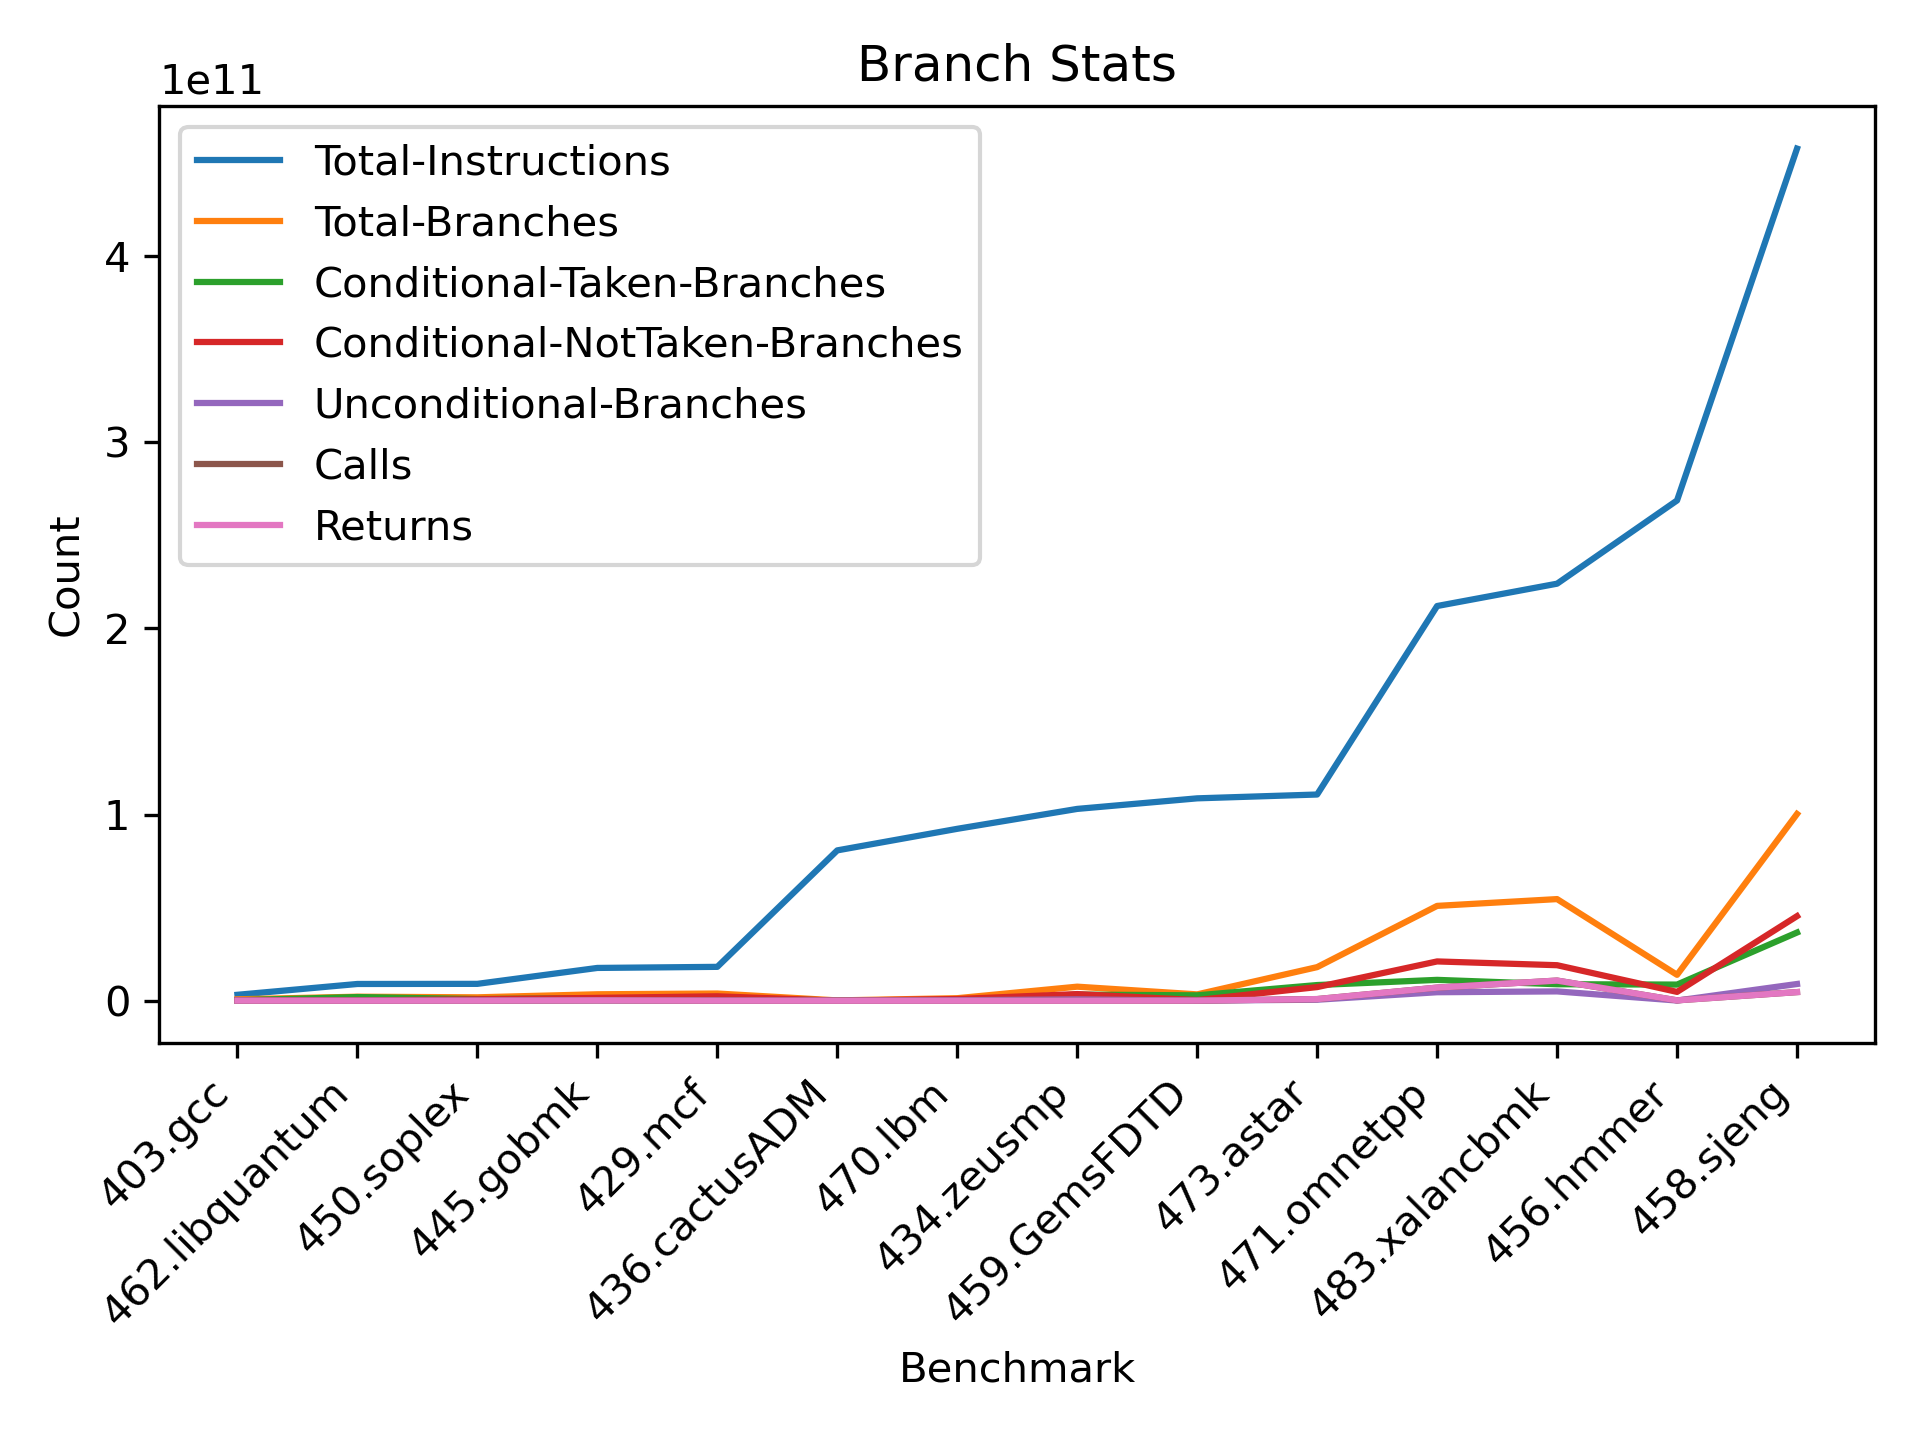
\includegraphics[width=0.6\textwidth]{./outputs/branch_stats.png} 
    \caption{Στατιστικά στοιχεία εντολών διακλάδωσης μετροπρογραμμάτων}
    \label{fig:branch_stats}
\end{figure}
\FloatBarrier

Τα μετροπρογράμματα στον οριζόντιο άξονα είναι ταξινομημένα βάσει του πλήθους των συνολικών εντολών. Φαίνεται, ότι η διακύμαση στο πλήθος εντολών είναι αρκετά μεγάλη. Ωστόσο, η διακύμανση στο πλήθος των εντολών δεν είναι το ίδιο εντόνη, αν και, δεδομένης της κλίμακας ($10^{11})$ παραμένει αρκετά υψηλή. Γενικώς, όσο αυξάνονται οι συνολικές εντολές, τόσο αυξάνονται και οι εντολές διακλάδωσεις, με εξαίρεση το μετροπρόγραμμα \eng{\texttt{456.hmmer}}, το οποίο έχει λιγότερες διακλάδωσεις από το αναμενόμενο. Οι δε διάφορες κατηγορίες των διακλαδώσεων ακολουθούν την ίδια κατανομή με τις συνολικές διακλαδώσεις.

\clearpage
\section{Μελέτη των \eng{N-bit Predictors}}

\subsection{\eng{Hardware 16K}}

Παρατίθεται γράφημα το οποίο παρουσιάζει την επίδοση των διαφόρων \eng{N-bit predictors} ανά μετροπρόγραμμα.

\begin{figure}[h]
    \centering
    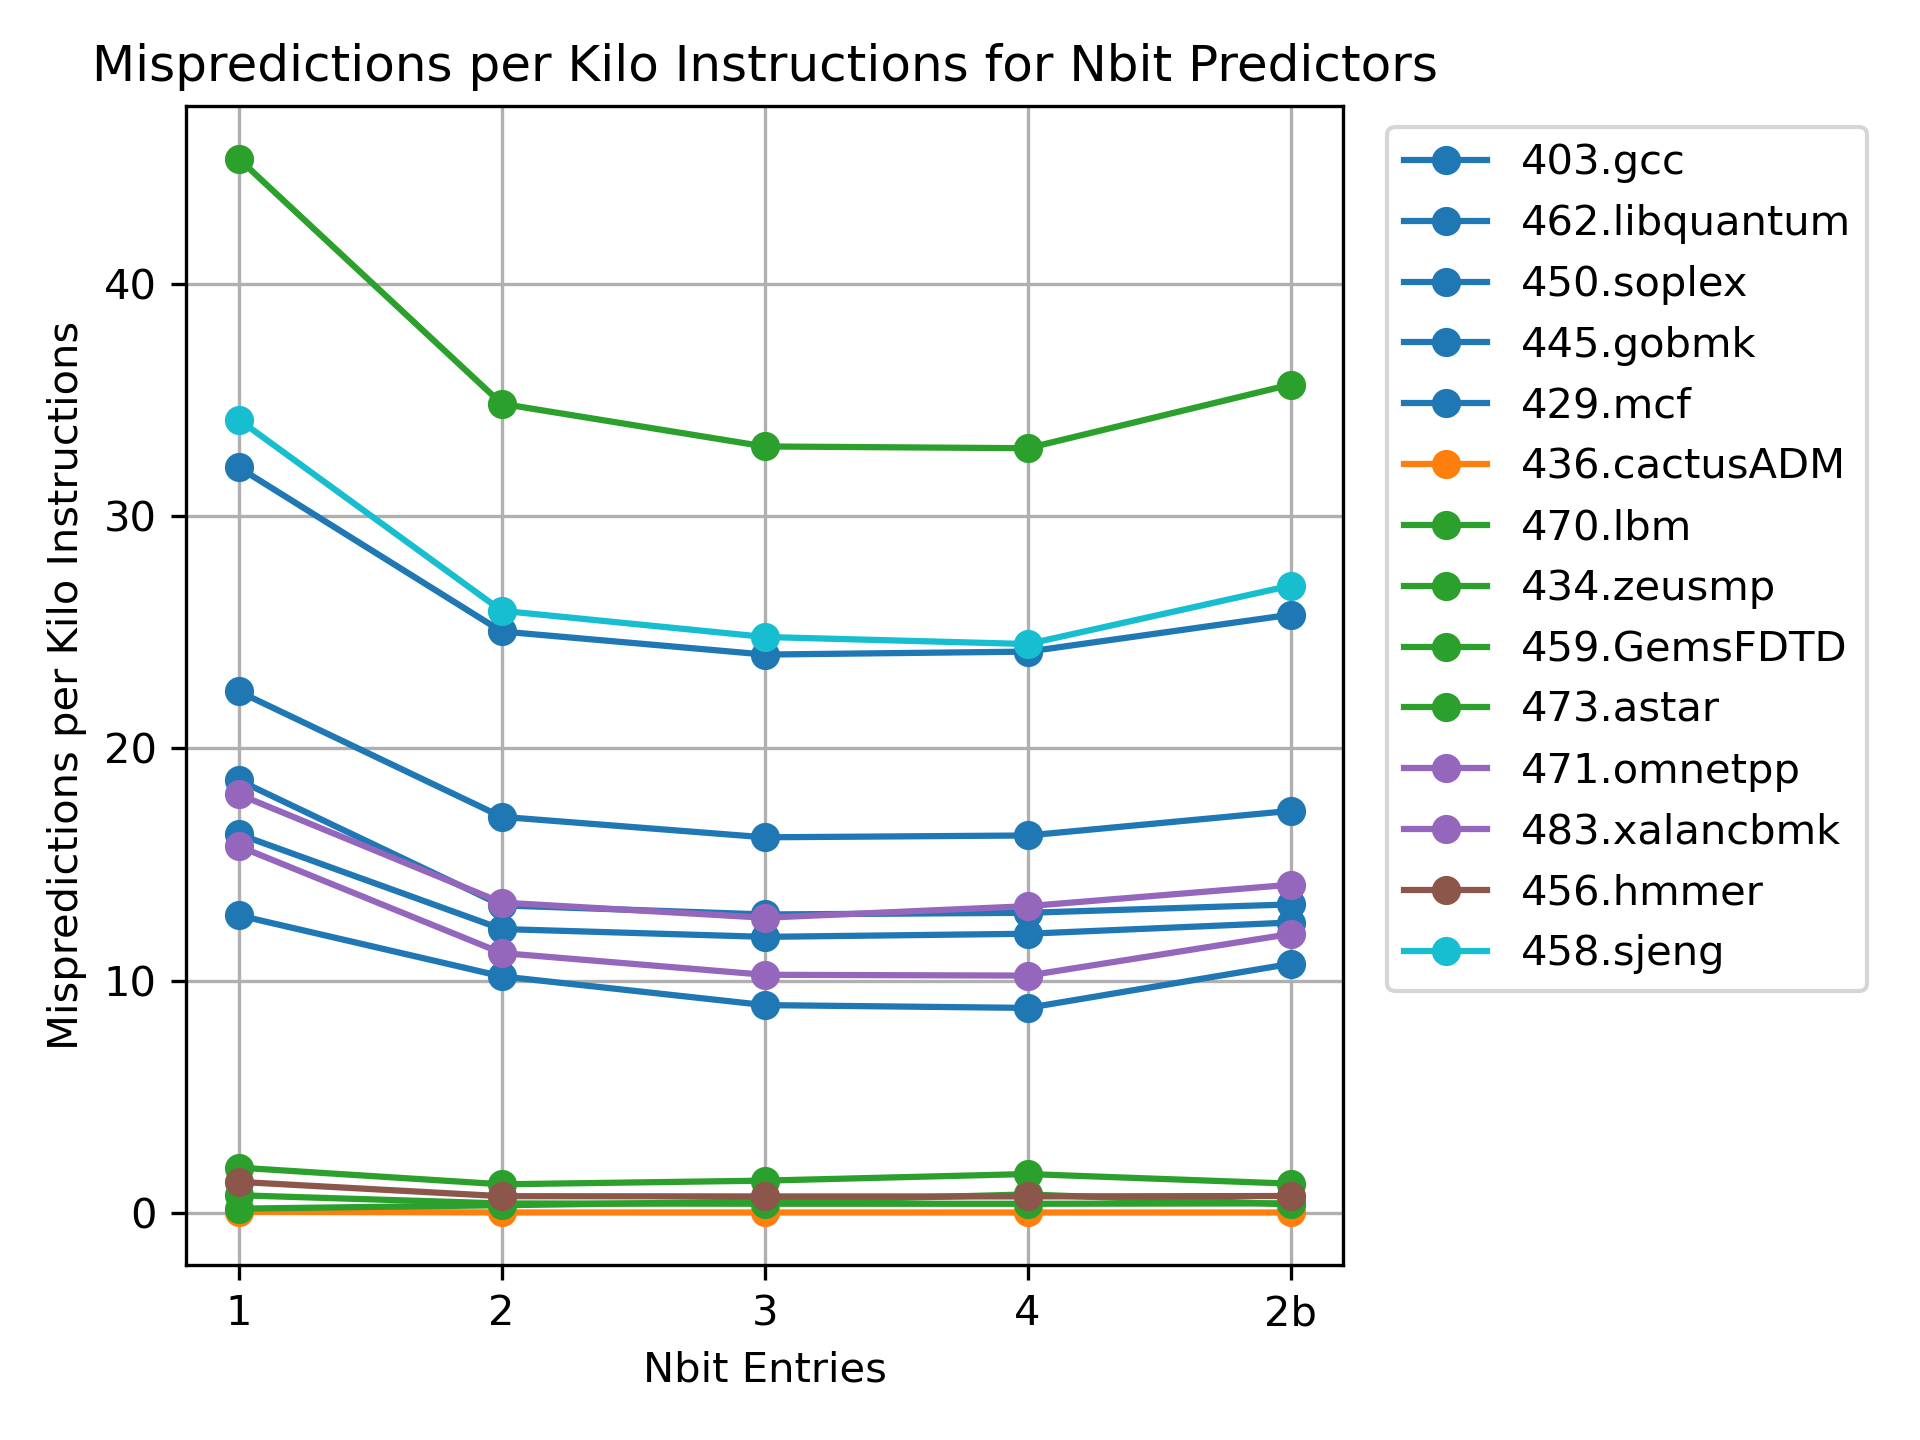
\includegraphics[width=0.6\textwidth]{./outputs/nbit16k.png} 
    \caption{Επίδοση διαφόρων \eng{N-bit predictors 16K} ανά μετροπρόγραμμα}
    \label{fig:nbit16k}
\end{figure}
\FloatBarrier

Φαίνεται, ότι, γενικώς, η σχετική επίδοση των \eng{predictors} μεταξύ τους είναι παρόμοια. Δηλαδή, η χείριστη επίδοση επιτυγχάνεται με τον προβλέπτη του ενός \eng{bit} και η βέλτιστη με τον προβλέπτη των τεσσάρων \eng{bits}. Σημειώνεται, ότι στα μετροπρογράμματα στα οποία οι αστοχίες είναι ελάχιστες, επιτυγχάνεται βέλτιστη επίδοση από τους προβλέπτες δύο \eng{bit} και χείριστη από αυτούς των τεσσάρων και του ενός \eng{bit}. 

Παρατηρείται, επίσης, αρκετά μεγάλη διακύμανση στο ποσοστό των αστοχιών ανά 1000 εντολές. Αν διερευνηθεί το σχήμα \ref{fig:branch_stats}, μπορεί να διαπιστωθεί ότι το πολύ χαμηλό \eng{mpki} επιτυγχάνεται από τα μετροπρογράμματα τα οποία παρουσιάσαν αύξηση στο πλήθος εντολών χωρίς να παρουσιάσουν αύξηση στο πλήθος εντολών διακλάδωσης. Ομοίως, στο μέσον του κατακορύφου άξονα στο σχήμα \ref{fig:nbit16k} εντοπίζονται τα μετροπρογράμματα, τα οποία παρουσίασαν ανάλογη αύξηση των εντολών διακλάδωσης με τις συνολικές εντολές. Γενικώς, αυτή η έντονη διαφορά στο \eng{mpki} αιτιολογείται από τον λόγο των εντολών διακλάδωσης ως προς τις συνολικές εντολές. 

\subsection{\eng{Hardware 32K}}

Παρατίθεται γράφημα το οποίο παρουσιάζει την επίδοση των διαφόρων \eng{N-bit predictors} ανά μετροπρόγραμμα. Αυτήν την φορά παραλείπεται ο προβλέπτης των τριών \eng{bits} και διατηρούνται οι υπόλοιποι.

Αρχικά, σημειώνεται, ότι η παραλλαγή του προβλέπτη δύο \eng{bits} εμφανίζεται πριν τον προβλέπτη των τεσσάρων και όχι μετά όπως προηγουμένως. Με αυτό κατά νου, παρατηρείται ότι η συμπεριφορά των προβλέπτων παραμένει γενικώς ίδια. Συγκεκριμένα, τόσο η σχετική τους επίδοση όσο και τα απόλυτα ποστοστά τους παραμένουν αρκετά όμοια με προηγουμένως. Αυτό οδηγεί στο συμπέρασμα ότι ο διπλασιασμός των καταχωρήσεων, από 16Κ σε 32Κ, δεν συμβάλει καθοριστικά στην επίδοση των προβλέπτων. 

\begin{figure}[h]
    \centering
    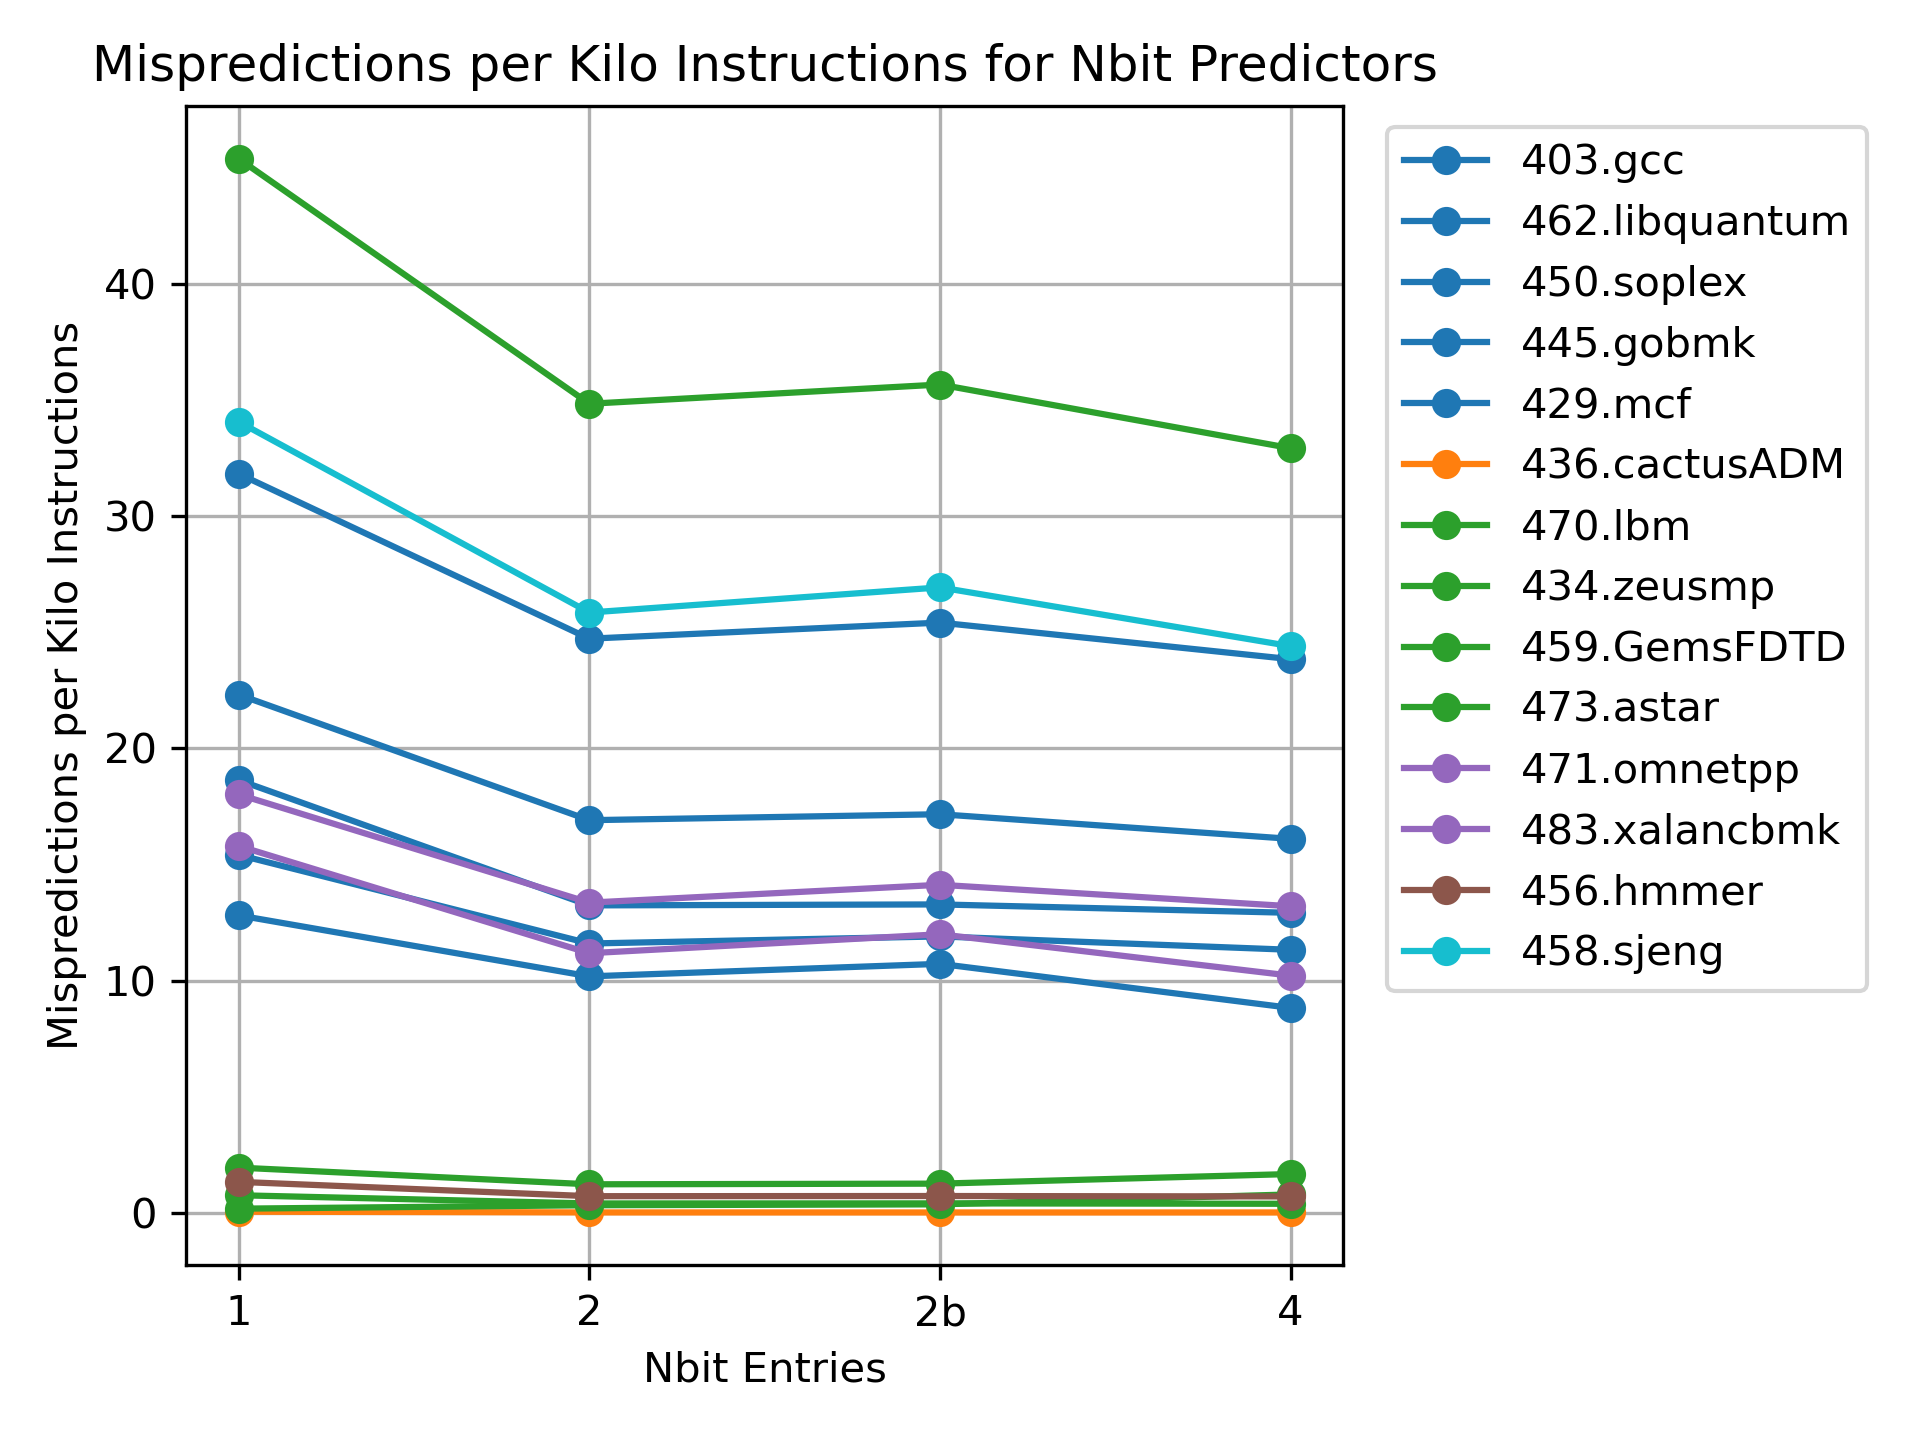
\includegraphics[width=0.6\textwidth]{./outputs/nbit32k.png} 
    \caption{Επίδοση διαφόρων \eng{N-bit predictors 32K} ανά μετροπρόγραμμα}
    \label{fig:nbit32k}
\end{figure}
\FloatBarrier

Ως βέλτιστη επιλογή επιλέγεται ο προβλέπτης των τεσσάρων \eng{bits}, αφού γενικά φαίνεται να αποδίδει καλύτερα. 

\clearpage
\section{Μελέτη του \eng{BTB}}

Παρατίθεται γράφημα με την επίδοση του \eng{Branch Target Buffer} για διάφορα πλήθη καταχωρήσεων και συσχετιστικοτήτων.

Παρατηρείται, ότι η συμπεριφορά ανά μετροπρόγραμμα είναι όμοια. Φαίνεται, ότι η επίδοση του \eng{Branch Target Buffer} δεν παρουσιάζει πολλές διακυμάνσεις. Οι πρώτες 4 διατάξεις, με την διπλάσια χωρητικότητα από τις επόμενες 4, φαίνονται να αποδίδουν ελαφρώς καλύτερα. Μεταξύ τους, την βέλτιστη επίδοση φαίνεται να την έχει η διάταξη με την υψηλότερη συσχετιστικότητα. Επομένως, ως καλύτερη οργάνωση για το \eng{BTB} επιλέγεται η οργάνωση \eng{(lines, assoc) = (256, 4)}.

\begin{figure}[h]
    \centering
    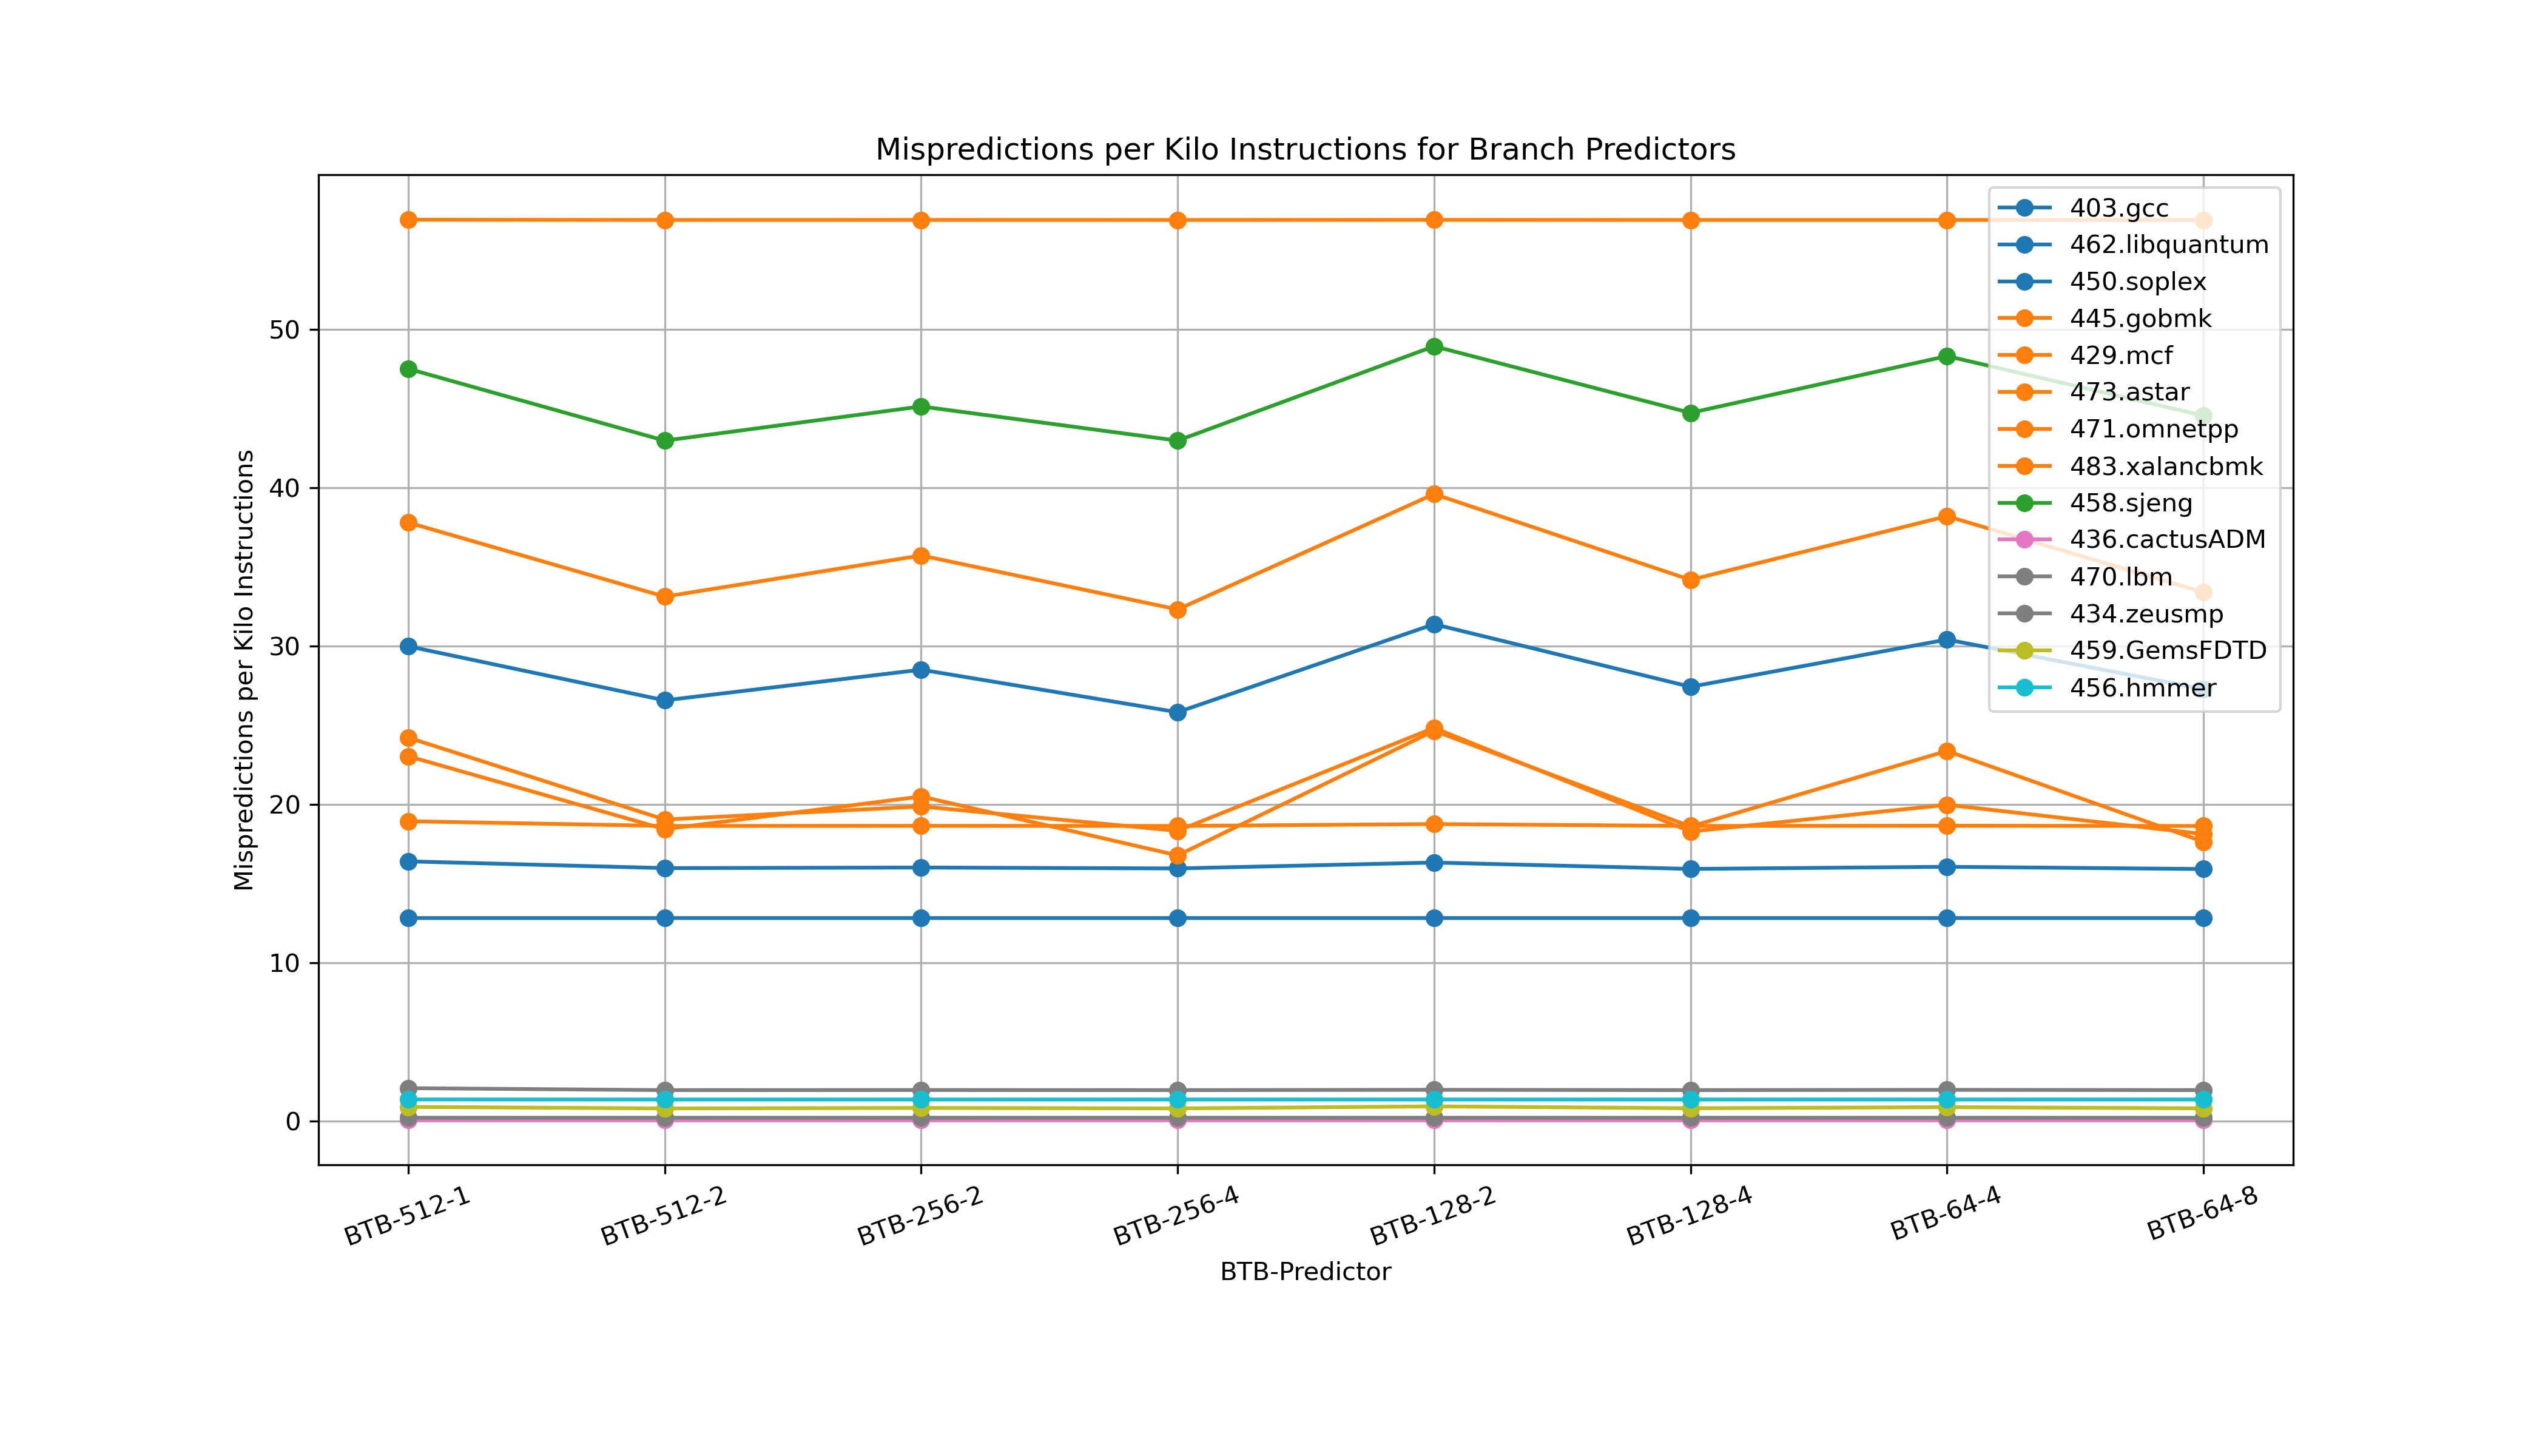
\includegraphics[width=\textwidth]{./outputs/btb.png} 
    \caption{Επίδοση διαφόρων \eng{Branch Target Buffer} ανά μετροπρόγραμμα}
    \label{fig:btb}
\end{figure}
\FloatBarrier

\clearpage
\section{Μελέτη του \eng{RAS}}

Παρατίθεται γράφημα με την επίδοση του \eng{Return Address Stack} για διάφορα πλήθη καταχωρήσεων.

\begin{figure}[h]
    \centering
    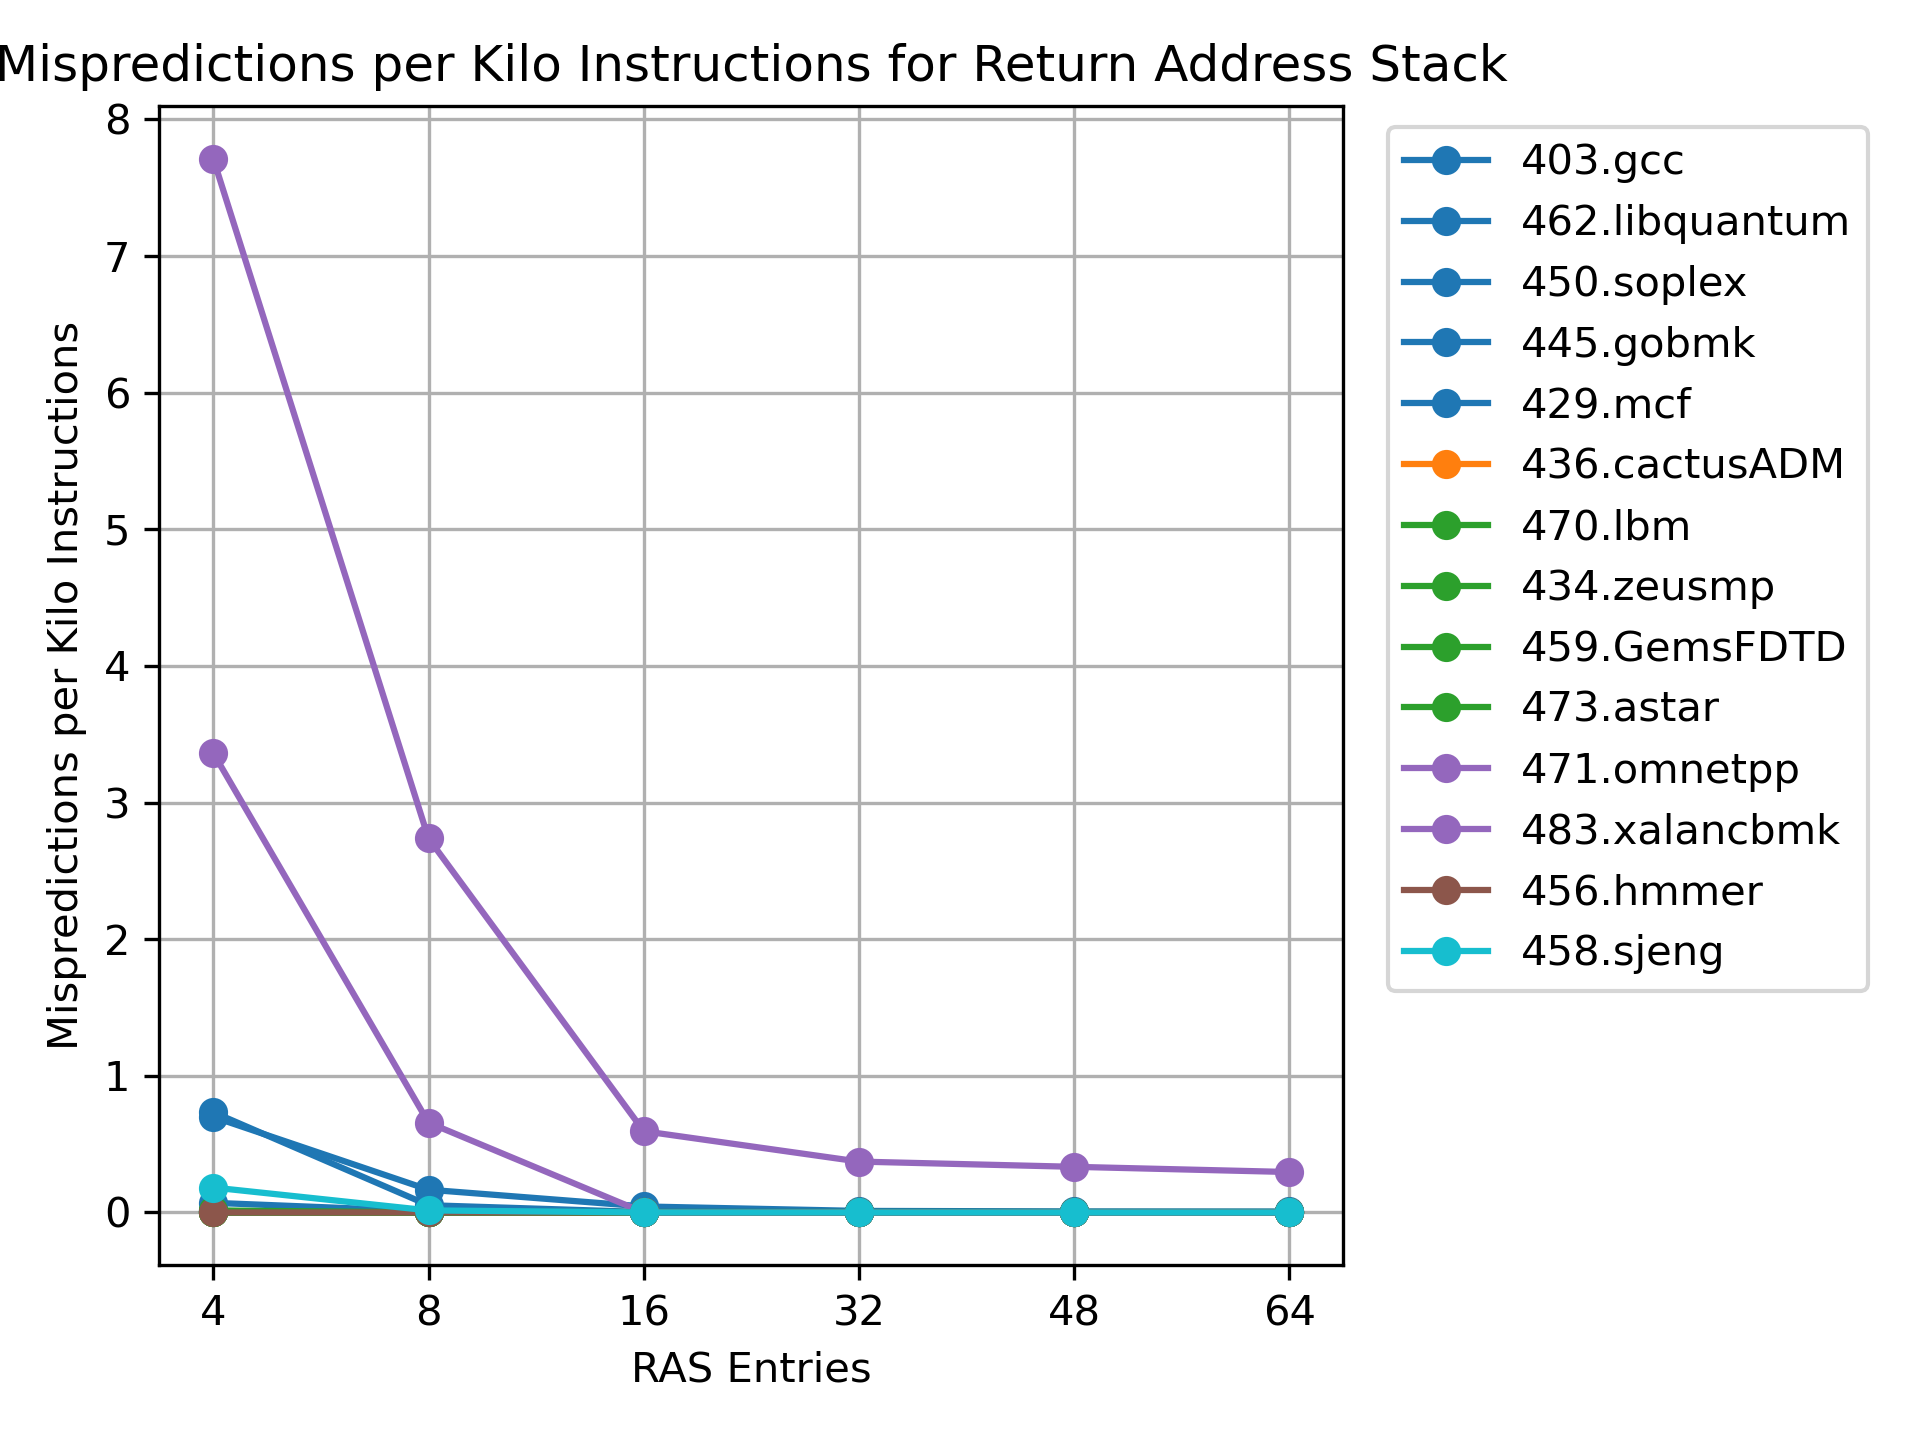
\includegraphics[width=0.6\textwidth]{./outputs/ras.png} 
    \caption{Επίδοση διαφόρων \eng{Return Address Stack} ανά μετροπρόγραμμα}
    \label{fig:ras}
\end{figure}
\FloatBarrier

Αρχικά, παρατηρείται η ίδια συμπεριφορά σε όλα τα προγράμματα. Φαίνεται σαφώς, ότι όσο αυξάνεται το μέγεθος της στίβας, τόσο αυξάνεται η απόδοση, δηλαδή μειώνεται το \eng{mpki}. Μάλιστα, αυτό συμβαίνει εκθετικά, με την απόδοση να φτάνει πολύ κόντα στο βέλτιστο από τις 16 καταχωρίσεις και μετά, με λίγη διαφορά μέχρι τις 64 καταχωρίσεις. Ως κατάλληλο μέγεθος, λοιπόν, επιλέγονται οι 64 καταχωρίσεις. 

\clearpage
\section{Σύγκριση Διαφορετικών \eng{predictors}}

Παρατίθεται πρώτα το γράφημα για την απόδοση των διαφόρων προβλέπτων. Δοκιμάστηκαν 22 προβλέπτες, μεταξύ των οποίων ήταν στατικοί, \eng{N-bit predictors}, \eng{Local History predictors}, \eng{Global history predictors} και διάφοροι \eng{Tournament predictors}, εκ των οποίων και ο \eng{alpha 21264}. Αν και παρατίθενται όλοι στο γράφημα, φάνηκε δύσκολο να τυπωθούν ικανοποιητικά τα αποτελέσματα, άρα παρατίθεται ενδεικτικά και ένα αρχείο εξόδου με τα ονόματά τους. 

\begin{figure}[h]
    \selectlanguage{english}
    \verbatiminput{outputs\_original/showdown/403.gcc.cslab\_branch\_predictors.out}
    \selectlanguage{greek}
    \caption{Έξοδος \eng{403.gcc.cslab\_branch\_predictors.out}}
\end{figure}
\FloatBarrier


\begin{figure}[h]
    \centering
    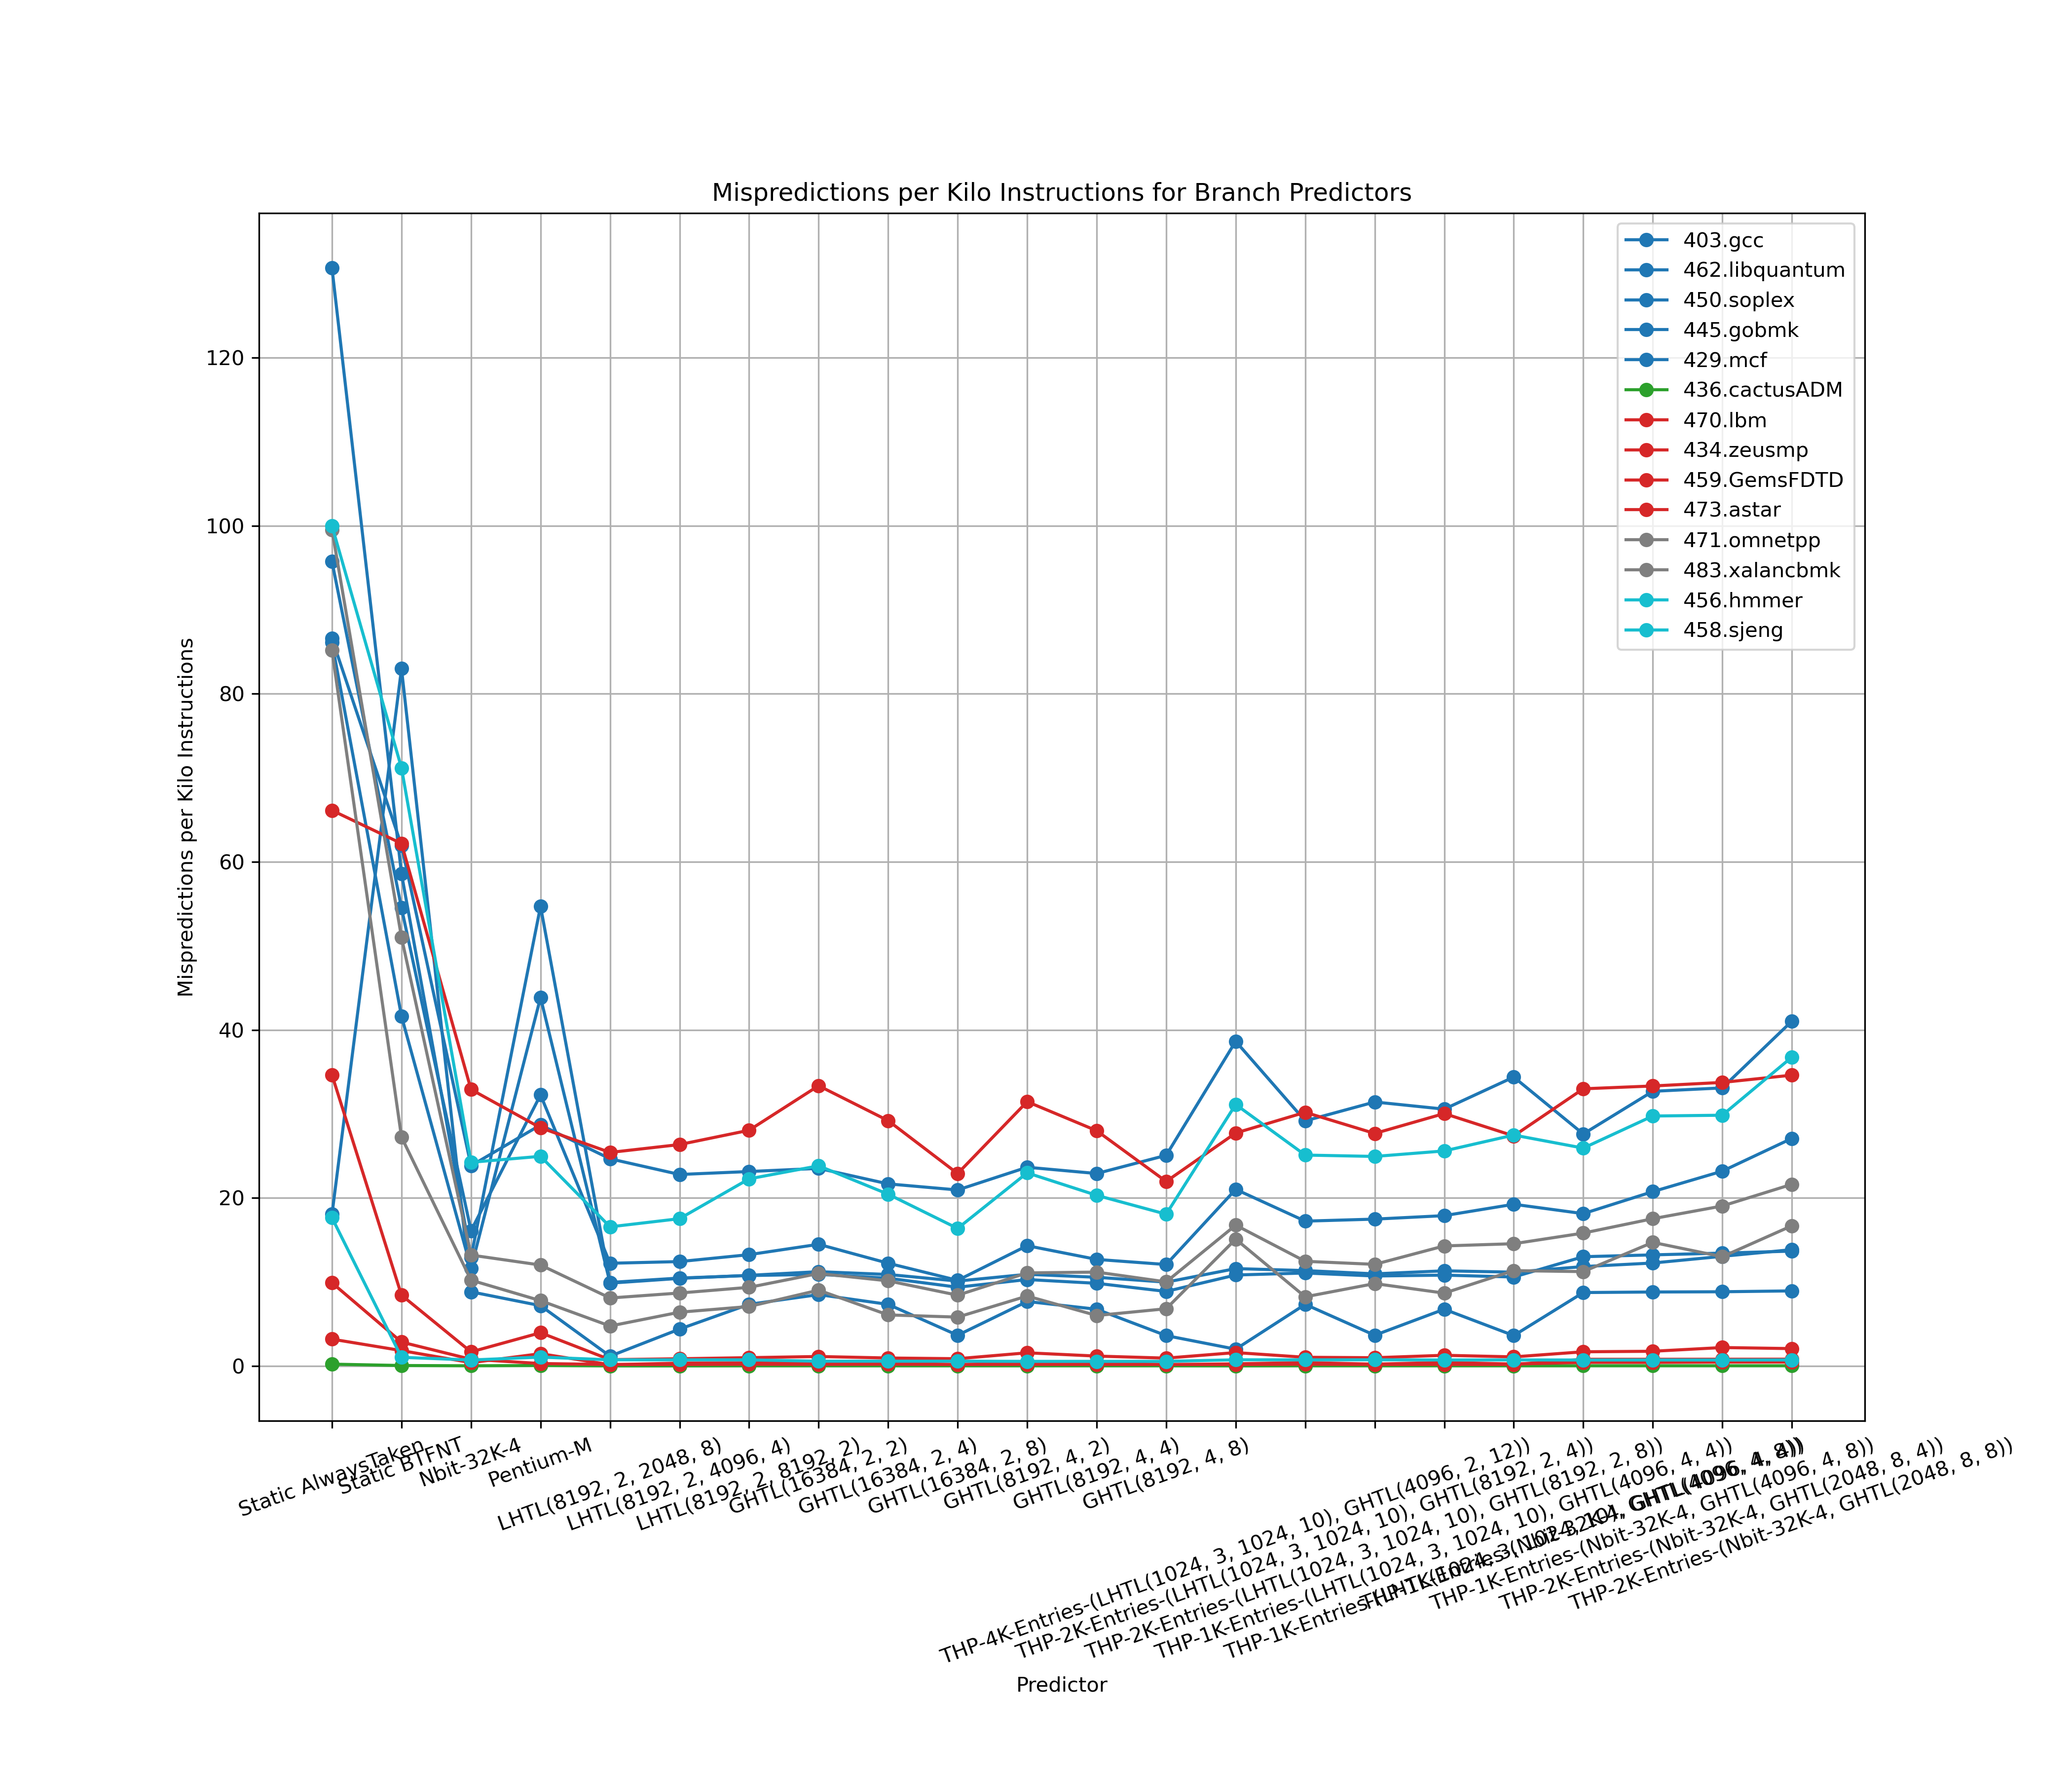
\includegraphics[width=\textwidth]{./outputs/showdown.png} 
    \caption{Επίδοση διαφόρων \eng{predictors} ανά μετροπρόγραμμα}
    \label{fig:showdown}
\end{figure}
\FloatBarrier

Αρχικά, παρατηρείται ότι οι στατικοί προβλέπτες είναι αρκετά κακοί, πράγμα αναμενόμενο, αφού δεν προσαρμόζονται καθόλου δυναμικά στον εκτελούμενο κώδικα αλλά ``προβλέπουν'' βάσει μίας παγειωμένης απόφασης. Ο \eng{Pentium M} επίσης δεν αποδίδει καλά, καθώς σε όλα τα μετροπρογράμματα παρουσιάζει χειρότερη απόδοση, τόσο από τον \eng{N-bit predictor} όσο και από τους \eng{local} και \eng{global history predictors}.

Μεταξύ των \eng{local / global history predictors}, την βέλτιστη απόδοση παρουσιάζουν οι \eng{global history two level predictors} με το μεγαλύτερο ιστορικό \eng{BHR length = 8}. Άρα, φαίνεται να είναι αυτός ο καθοριστικός παράγοντας για την απόδοσή τους, και όχι τόσο το πλήθος των καταχωρήσεων ή τα \eng{bits} των προβλέπτων / μετρητών που χρησιμοποιούνται σε κάθε καταχώριση. Το ίδιο συμπέρασμα μπορεί να εξαχθεί και από τις αποδόσεις των τριών \eng{local history predictors}.  

Σχετικά με τους \eng{tournament predictors}, ο προβλέπτης \eng{alpha 21264} παρουσιάζει χειρότερη απόδοση στα περισσότερα μετροπρογράμματα, με εξαίρεση λίγα. Αυτό ίσως αιτιολογείται και από το γεγονώς, ότι δεν χρησιμοποιεί καθόλου την διεύθυνση της εντολής διακλάδωσης για την πρόβλεψη του \eng{local history two level predictor}, αλλά χρησιμοποιεί μόνο το ιστορικό \eng{BHR length = 12}. Οι \eng{tournament predictors} με \eng{n-bit predictors} παρουσίασαν χειρότερη απόδοση από τους υπόλοιπους. Βέβαια, δεν δοκιμάστηκαν μαζί με \eng{local history predictors}, άρα δεν μπορεί να εξαχθεί σαφές συμπέρασμα από τις παρούσες μετρήσεις. Γενικά, μεταξύ των \eng{tournament predictors}, την βέλτιστη απόδοση φαίνεται να έχουν όσοι συνδυάζουν \eng{local history predictor} και \eng{global history predictor}, και μάλιστα με μεγάλα \eng{BHR Length}.

Συμπερασματικά, το βέλτιστο αποτέλεσμα παρουσιάσαν οι προβλέπτες οι οποίοι περιείχαν προβλέπτη \eng{global history two level predictor} με \eng{BHR Length = 8}. Άρα, οποιοσδήποτε από τους:

\begin{itemize}
    \item \eng{GHTL(8192, 4, 8)}
    \item \eng{GHTL(16384, 2, 8)}
    \item \eng{THP-2K-(LHTL(1024, 3, 1024, 10), GHTL(8192, 2, 8))}
    \item \eng{THP-1K-(LHTL(1024, 3, 1024, 10), GHTL(4096, 4, 8))}
\end{itemize} μπορεί να επιλεχθεί ως βέλτιστος. Στην παρούσα εργασία επιλέγεται ο τελευταιός γιατί έχει τις ελάχιστες καταχωρήσεις και επομένως το λιγότερο υλικό, αν και η διαφορά είναι μικρή. 

\clearpage
\section{Παράρτημα}
\subsection{\eng{TwoBitBPredictor}}
\selectlanguage{english}
\begin{lstlisting}[style=Cstyle]
    class TwobbitPredictor: public BranchPredictor
    {
    public:
        TwobbitPredictor(unsigned index_bits_)
        : BranchPredictor(), index_bits(index_bits_) {
            table_entries = 1 << index_bits;
            TABLE = new unsigned long long[table_entries];
            memset(TABLE, 0, table_entries * sizeof(*TABLE));

            COUNTER_MAX = (1 << 2) - 1;
        };

        ~TwobbitPredictor() { delete TABLE; };

        virtual bool predict(ADDRINT ip, ADDRINT target) {
            unsigned int ip_table_index = ip % table_entries;
            unsigned long long ip_table_value = TABLE[ip_table_index];
            unsigned long long prediction = ip_table_value >> (2 - 1);
            return (prediction != 0);
        };

        virtual void update(bool predicted, bool actual, ADDRINT ip, ADDRINT target) {
            unsigned int ip_table_index = ip % table_entries;
            if (actual) {
                if (TABLE[ip_table_index] == 0)
                TABLE[ip_table_index]++;
                else TABLE[ip_table_index] = COUNTER_MAX;
            } else {
                if (TABLE[ip_table_index] == COUNTER_MAX)
                TABLE[ip_table_index]--;
                else TABLE[ip_table_index] = 0;
            }

            updateCounters(predicted, actual);
        };

        virtual string getName() {
            std::ostringstream stream;
            stream << "Nbit-" << pow(2.0,double(index_bits)) / 1024.0 << "K-" << 2 << 'b';
            return stream.str();
        }

    private:
        unsigned int index_bits;
        unsigned int COUNTER_MAX;

        /* Make this unsigned long long so as to support big numbers of cntr_bits. */
        unsigned long long *TABLE;
        unsigned int table_entries;
    };
\end{lstlisting}
\clearpage
\subsection{\eng{BTB}}
\begin{lstlisting}[style=cstyle]    
class BTBPredictor : public BranchPredictor
{
public:
	BTBPredictor(int btb_lines, int btb_assoc)
    : table_lines(btb_lines), table_assoc(btb_assoc),
    correct_target_predictions(0), incorrect_target_predictions(0), timestamp(0)
	{
        total = table_lines*table_assoc;
		btb.resize(total);
        for (int i = 0; i < table_lines; i++) {
			btb[i].resize(table_assoc, std::make_tuple(0, 0, 0));
		}
	}

	~BTBPredictor() { btb.clear(); }

    virtual bool predict(ADDRINT ip, ADDRINT target)
    {
        int index = ip % table_lines;
		for (auto &entry : btb[index])
        {
			if (std::get<0>(entry) == ip)
            {
                std::get<2>(entry) = timestamp++;
                return std::get<1>(entry) == target;
            }
		}
		return false;
	}

    virtual void update(bool predicted, bool actual, ADDRINT ip, ADDRINT target) {
		int index = ip % table_lines;
        if (actual && predicted)
        {
            for (auto &entry : btb[index])
            {
                if (std::get<0>(entry) == ip)
                {
                    correct_target_predictions += (std::get<1>(entry) == target);
                    incorrect_target_predictions += (std::get<1>(entry) != target);
                    std::get<1>(entry) = target;
                }
            }
        }
		// if not found, replace the least recently used entry
        else if (actual && !predicted)
        {
            int min = 0;
            for (int i = 0; i < table_assoc; i++)
            {
                if (std::get<2>(btb[index][i]) < std::get<2>(btb[index][min]))
                    min = i;
            }
            std::get<0>(btb[index][min]) = ip;
            std::get<1>(btb[index][min]) = target;
            std::get<2>(btb[index][min]) = timestamp++;
        }
        else if (!actual && predicted)
        {
            for (auto &entry: btb[index])
            {
                if (std::get<0>(entry) == ip)
                {
                    std::get<0>(entry) = 0;
                    std::get<1>(entry) = 0;
                    std::get<2>(entry) = 0;
                }
            }
        }
        updateCounters(predicted, actual);
	}

    virtual string getName() {
        std::ostringstream stream;
		stream << "BTB-" << table_lines << "-" << table_assoc;
		return stream.str();
	}

    UINT64 getNumCorrectTargetPredictions() { return correct_target_predictions; }
	UINT64 getNumIncorrectTargetPredictions() { return incorrect_target_predictions; }

private:
	int table_lines, table_assoc, total;
    UINT64 correct_target_predictions;
    UINT64 incorrect_target_predictions;
    UINT64 timestamp;
    // The Branch Target Buffer
    // Each entry is a tuple of (ip, target, counter)
    // the counter is used in order to implement LRU replacement
	std::vector<std::vector<std::tuple<ADDRINT, ADDRINT, UINT64>>> btb;
};
\end{lstlisting}
\clearpage
\subsection{\eng{StaticAlwaysTaken and StaticBTFNT Predictors}}
\begin{lstlisting}[style=Cstyle]
    class StaticAlwaysTakenPredictor: public BranchPredictor
    {
    public:
        StaticAlwaysTakenPredictor(): BranchPredictor() {};

        ~StaticAlwaysTakenPredictor() {};

        virtual bool predict(ADDRINT ip, ADDRINT target)
        {
            return true;
        };

        virtual void update(bool predicted, bool actual, ADDRINT ip, ADDRINT target)
        {
            updateCounters(predicted, actual);
        };

        virtual string getName()
        {
            std::ostringstream stream;
            stream << "Static AlwaysTaken";
            return stream.str();
        }
    };
\end{lstlisting}
\begin{lstlisting}[style=Cstyle]
    class StaticBTFNTPredictor: public BranchPredictor
    {
    public:
        StaticBTFNTPredictor(): BranchPredictor() {};

        ~StaticBTFNTPredictor() {};

        virtual bool predict(ADDRINT ip, ADDRINT target)
        {
            return (target < ip);
        };

        virtual void update(bool predicted, bool actual, ADDRINT ip, ADDRINT target)
        {
            updateCounters(predicted, actual);
        };

        virtual string getName()
        {
            std::ostringstream stream;
            stream << "Static BTFNT";
            return stream.str();
        }
    };
\end{lstlisting}
\clearpage
\subsection{\eng{LocalHistoryTwoLevel Predictor}}
\begin{lstlisting}[style=Cstyle]
    class LocalHistoryTwoLevelPredictor: public BranchPredictor
    {
    public:
        LocalHistoryTwoLevelPredictor(unsigned int pht_bits_, unsigned int pht_entries_,
        unsigned int bht_bits_, unsigned int bht_entries_)
        : BranchPredictor(), pht_bits(pht_bits_), bht_bits(bht_bits_), pht_entries(pht_entries_), bht_entries(bht_entries_)
        {
            COUNTER_MAX = (1 << pht_bits) - 1;
            CAP = 1 << bht_bits;
            BHT = new unsigned long long [bht_entries];
            memset(BHT, 0, bht_entries * sizeof(*BHT));
            PHT = new unsigned long long [pht_entries];
            memset(PHT, 0, pht_entries * sizeof(*PHT));
        };

        ~LocalHistoryTwoLevelPredictor()
        {
            delete BHT;
            delete PHT;
        };

        virtual bool predict(ADDRINT ip, ADDRINT target)
        {
            unsigned int bht_table_index = ip % bht_entries;
            unsigned long long bht_table_value = BHT[bht_table_index];
            unsigned long long pht_table_index = (((ip % pht_entries) << (bht_bits)) + bht_table_value) % pht_entries;
            unsigned long long prediction = (PHT[pht_table_index] >> (pht_bits - 1));
            return (prediction != 0);
        };

        virtual void update(bool predicted, bool actual, ADDRINT ip, ADDRINT target)
        {
            unsigned int bht_table_index = ip % bht_entries;
            unsigned long long bht_table_value = BHT[bht_table_index];
            unsigned long long pht_table_index = (((ip % pht_entries) << (bht_bits)) + bht_table_value) % pht_entries;
            if (actual) {  // update pht for specific pattern
                if (PHT[pht_table_index] < COUNTER_MAX)
                PHT[pht_table_index]++;
            } else {
                if (PHT[pht_table_index] > 0)
                PHT[pht_table_index]--;
            }
            // update bht for specific branch
            BHT[bht_table_index] = ((actual << bht_bits) + BHT[bht_table_index]) >> 1;
            updateCounters(predicted, actual);
        };

        virtual string getName()
        {
            std::ostringstream stream;
            stream << "LocalHistoryTwoLevel: PHT Entries = " << pht_entries
            << ", PHT n-bit counter length = " << pht_bits
            << ", BHT Entries = " << bht_entries
            << ", BHT Entry length = " << bht_bits;
            return stream.str();
        }
    private:
        unsigned int pht_bits, bht_bits, pht_entries, bht_entries, COUNTER_MAX, CAP;;
        unsigned long long *BHT,*PHT;
    };
\end{lstlisting}
\clearpage
\subsection{\eng{GlobalHistoryTwoLevel Predictor}}
\begin{lstlisting}[style=Cstyle]
    class GlobalHistoryTwoLevelPredictor: public BranchPredictor
    {
    public:
        GlobalHistoryTwoLevelPredictor(unsigned int pht_entries_, unsigned int pht_bits_, unsigned int bhr_length_)
        : BranchPredictor(), pht_bits(pht_bits_), pht_entries(pht_entries_), bhr_length(bhr_length_)
        {
            COUNTER_MAX = (1 << pht_bits) - 1;
            BHR = 0;
            PHT = new unsigned long long [pht_entries];
            memset(PHT, 0, pht_entries * sizeof(*PHT));
        };

        ~GlobalHistoryTwoLevelPredictor()
        {
            delete PHT;
        };

        virtual bool predict(ADDRINT ip, ADDRINT target)
        {
            unsigned int pht_table_index = ((BHR * (pht_entries >> bhr_length)) + (ip % (pht_entries >> bhr_length))) % pht_entries;
            unsigned long long pht_table_value = PHT[pht_table_index];
            unsigned long long prediction = (pht_table_value >> (pht_bits - 1));
            return (prediction != 0);
        };

        virtual void update(bool predicted, bool actual, ADDRINT ip, ADDRINT target)
        {
            unsigned int pht_table_index = ((BHR * (pht_entries >> bhr_length)) + (ip % (pht_entries >> bhr_length))) % pht_entries;
            // update pht for specific pattern
            if (actual) {
                if (PHT[pht_table_index] < COUNTER_MAX)
                PHT[pht_table_index]++;
            } else {
                if (PHT[pht_table_index] > 0)
                PHT[pht_table_index]--;
            }
            // update bhr
            // shift the prediction to the left by history length bits
            // add it to the register (it's like you are queuing the prediction)
            // and then shift the whole thing to the right by one bit.
            BHR = ((actual << bhr_length) + BHR) >> 1;
            updateCounters(predicted, actual);
        };

        virtual string getName()
        {
            std::ostringstream stream;
            stream << "GlobalHistoryTwoLevel: PHT Entries = " << pht_entries
            << ", PHT n-bit counter length = " << pht_bits
            << ", BHR Length = " << bhr_length;
            return stream.str();
        };

    private:
        unsigned int pht_bits, pht_entries, bhr_length;
        unsigned int COUNTER_MAX;
        unsigned long long BHR;
        unsigned long long *PHT;
    };
\end{lstlisting}
\clearpage
\subsection{\eng{TournamentHybrid Predictor}}
\begin{lstlisting}[style=Cstyle]
    class TournamentHybridPredictor: public BranchPredictor
    {
    public:
        TournamentHybridPredictor(unsigned int meta_entries_, unsigned int cntr_bits_, BranchPredictor* p0, BranchPredictor* p1)
        : meta_entries(meta_entries_), cntr_bits(cntr_bits_), predictor0(p0), predictor1(p1)
        {
            TABLE = new unsigned long long[meta_entries];
            memset(TABLE, 0, meta_entries * sizeof(*TABLE));
            COUNTER_MAX = (1 << cntr_bits) - 1;
        };
        ~TournamentHybridPredictor() {delete TABLE;};
        virtual bool predict(ADDRINT ip, ADDRINT target) {
            unsigned int ip_table_index = ip % meta_entries;
            unsigned long long ip_table_value = TABLE[ip_table_index];
            bool predictor = ip_table_value >> (cntr_bits - 1);
            prediction0 = predictor0->predict(ip, target);
            prediction1 = predictor1->predict(ip, target);
            return (!predictor)*(prediction0) + (predictor)*(prediction1);
        };

        virtual void update(bool predicted, bool actual, ADDRINT ip, ADDRINT target) {
            updateCounters(predicted, actual);
            predictor0->update(prediction0, actual, ip, target);
            predictor1->update(prediction1, actual, ip, target);

            if (prediction0 == prediction1) return ;

            unsigned int ip_table_index = ip % meta_entries;
            if (actual == prediction0) {
                if (TABLE[ip_table_index] < COUNTER_MAX)
                TABLE[ip_table_index]++;
            } else {
                if (TABLE[ip_table_index] > 0)
                TABLE[ip_table_index]--;
            }
        };

        virtual string getName() {
            std::ostringstream stream;
            stream << "TournamentHybridPredictor-" << meta_entries / 1024.0 << "K-Entries-("
            << predictor0->getName() << ", " << predictor1->getName() << ")";
            return stream.str();
        }

    private:
        /* Make this unsigned long long so as to support big numbers of cntr_bits. */
        unsigned long long *TABLE;
        unsigned int meta_entries;
        unsigned int COUNTER_MAX, cntr_bits;
        BranchPredictor *predictor0;
        BranchPredictor *predictor1;
        bool prediction0, prediction1;
    };
\end{lstlisting}


\selectlanguage{greek}


\end{document}
